\section{Uniform lower comparison}\label{sec:lower}

We prove that the two cut constructions together separate every pair.
The common-bag estimate first puts a hypothetical collapsed pair into
a useful position relative to its least common ancestor bag. The anchor
retention rule will then contradict that collapse.

\begin{proposition}[Uniform lower comparison]\label{prop:combined-lower}
For each fixed $k\geq2$ there is a constant $\lambda_k>0$ such that, for
every admissible weighted graph with a tree decomposition of bag size
at most $k$ and every pair of vertices $u,v$,
\begin{equation}\label{eq:combined-lower}
 D_{\mathrm{bag}}(u,v)+D_{\mathrm{anc}}(u,v)
 \geq\lambda_k d(u,v).
\end{equation}
\end{proposition}

\subsection{Normalizing a failure of the lower bound}

To prove a uniform lower bound, we argue by contradiction from a normalized
sequence of poorly separated pairs. The bounded cache will yield a youngest
reservation crossing from distance bounded away from zero to vanishing
distance; the noise tests force geometric witnesses, and the eviction rule
then preserves a younger such reservation.

We give the limiting argument explicitly.  Fix a nonprincipal ultrafilter
$\mathcal U$ on $\mathbb N$, obtained by extending the cofinite filter
using Zorn's lemma.  An assertion about a sequence holds
\emph{eventually} if its set of valid indices belongs to $\mathcal U$;
sequences are identified when they agree eventually.  A \emph{standard}
constant means a fixed real number, independent of the sequence index.
A nonnegative real sequence is \emph{infinitesimal} if, for each $\varepsilon>0$, it is
eventually smaller than $\varepsilon$.  We will use only the following
elementary properties.

\begin{lemma}[Finite limiting rules]\label{lem:finite-limiting-rules}
\leavevmode
\begin{enumerate}
\item Of finitely many alternatives whose union holds eventually, at
least one holds eventually.  Finitely many eventual assertions hold
simultaneously eventually.
\item A sequence in $[0,1]$ that is not infinitesimal is eventually
bounded below by a positive real constant.  A finite minimum of such
sequences has the same property.
\item Sequences of times in finite linearly ordered paths are linearly
ordered modulo $\mathcal U$.  If $\delta_t\in[0,1]$ is nonincreasing
along each path, a time sequence with noninfinitesimal $\delta_t$
precedes every time sequence with infinitesimal $\delta_t$.
\end{enumerate}
\end{lemma}

\begin{proof}
The first assertion is the finite-union and finite-intersection property
of an ultrafilter.  If the second assertion failed, the sets on which the
sequence is smaller than each positive constant would all belong to
$\mathcal U$, which is exactly infinitesimality.  Take a finite minimum
of the resulting positive lower bounds to obtain its last claim.
For two time sequences, the alternatives $s<t$, $s=t$, and $s>t$
partition the indices, proving the ordering assertion.  If a time with
noninfinitesimal $\delta$ were at or after one with infinitesimal $\delta$,
monotonicity would bound its $\delta$ by an infinitesimal sequence, a
contradiction.
\end{proof}

Suppose, towards a contradiction, that the constructed sum
$D_{\mathrm{bag}}+D_{\mathrm{anc}}$ has no uniform positive lower
comparison with $d$.  Then there is a sequence of admissible metrics,
decompositions, and distinct pairs $x,y$, with $r=d(x,y)$, such that
\begin{equation}\label{eq:failed-lower-comparison}
 \frac{D_{\mathrm{bag}}(x,y)+D_{\mathrm{anc}}(x,y)}{r}
 \longrightarrow 0.
\end{equation}
All vertices, bags, metrics, and times in the rest of the argument denote
sequences in these examples; inequalities and temporal comparisons are
taken eventually unless stated otherwise. We write $a=o(b)$, for
positive sequences $b$, when $|a|/b$ tends to zero along $\mathcal U$;
in particular, $o(1)$ denotes an infinitesimal sequence. These choices
depend on the input metrics and the deterministic cache, not on the
sampled particles.

Choose bags containing the two endpoints and let $S$ be their least
common ancestor.  Every $x$--$y$ path meets $S$ by
Lemma~\ref{lem:separator}; in particular
\begin{equation}\label{eq:lca-distance-bound}
 d(x,S)\leq r,\qquad d(y,S)\leq r.
\end{equation}
The two ratios on the left divided by $r$ cannot both be infinitesimal.
Indeed, if $s,t\in S$ are respective nearest vertices, the upper bound
$D_{\mathrm{bag}}\leq U_{\mathrm{bag}}d$ would give
\[
 D_{\mathrm{bag}}(s,t)
 \leq U_{\mathrm{bag}}\bigl(d(x,S)+d(y,S)\bigr)
       +D_{\mathrm{bag}}(x,y)=o(r),
\]
whereas
$d(s,t)\geq r-d(x,S)-d(y,S)=(1-o(1))r$.
This contradicts the lower bound
$D_{\mathrm{bag}}(s,t)\geq a_{\mathrm{bag}}d(s,t)$ from
Proposition~\ref{prop:cobag}.

Interchange the endpoints, if necessary, so that $a=d(x,S)$ satisfies
$a/r\geq\varepsilon_0>0$ eventually.  Discard the irrelevant indices
where $a=0$, and divide each metric, particle height, and cut mass by
$a$.  We rescale the already constructed objects; no scale-equivariance
of a particular partition sampler is needed.  All their stated
inequalities and noise properties survive this change of units: the
functions $h_A,g_A,v_A$, bump amplitudes, and sweep cutoff are divided by
$a$, while the original independent uniform variables are unchanged.
The support and amplitude bounds in
Lemma~\ref{lem:ordinary-noise} therefore hold in the rescaled metric.
We use those bounds, without regenerating the partition samples or
requiring their original scales to remain dyadic.  Write
$D=D_{\mathrm{anc}}$ in the new units.  We have
\begin{equation}\label{eq:normalized-failure}
 d(x,S)=1,\qquad D(x,y)\text{ is infinitesimal},\qquad D\leq Ud.
\end{equation}

\subsection{A youngest crossing anchor}

Let $X$ be the chosen endpoint bag containing $x$, and consider the
descending path from $S$ to $X$.  Put $\delta_B=d(x,B)$.  By
Lemma~\ref{lem:separator}, these numbers are nonincreasing, lie in
$[0,1]$, and equal $1$ at $S$ and $0$ at $X$.  A selected sequence of
bags is called \emph{early} if its $\delta_B$ is not infinitesimal,
and \emph{late} otherwise.  An early sequence has a positive standard
lower bound for $\delta_B$; that bound may depend on the selected
sequence.  We never assume a first late bag or a last early bag exists.

For an anchor whose reservation meets this path, restrict its reservation
to the path, counting both launch and eviction bags and truncating at $X$
if it is not evicted earlier.  Its
effective start is its launch bag or $S$, whichever is later.  Call a
sequence of anchors \emph{crossing} if its effective start is early and
its terminal bag is late.  Equivalently, it has launched by an early
time and remains present at a late time.
Here an anchor sequence, like a time sequence, is an equivalence class
modulo equality on a set in $\mathcal U$.  Its launch time and terminal
time are defined by the deterministic cache, independently of the
particles sampled in its reservation.

\begin{lemma}[A youngest crossing anchor]\label{lem:youngest-crossing}
There are at most $n_0+1$ distinct crossing anchor sequences.  The set is
nonempty and has a youngest member $A_*$.
\end{lemma}

\begin{proof}
The permanent root is crossing.  Given any finite collection of crossing
anchor sequences, take their latest effective start.  It is early by
Lemma~\ref{lem:finite-limiting-rules}.  Every anchor in the collection
has started, and each of their late terminal times follows this early
time.  Thus they are simultaneously present in the inclusive cache list.
If $n_0+2$ distinct crossing sequences existed, select that many; their
pairwise distinctness also holds simultaneously eventually.  This would
contradict the bound $n_0+1$ of Lemma~\ref{lem:cache-defined}.
This bound concerns the set of equivalence classes of all crossing
sequences, not just a list chosen in advance.
The finite nonempty set of crossing anchors is ordered by launch time,
so it has a youngest member.
\end{proof}

Fix $A_*$ and write
\[
 h_*=d(\,\cdot\,,A_*),\qquad D_0=h_*(x).
\]
Choose its late terminal bag $Z$ and a nearest vertex $z\in Z$ to $x$.
Then $d(x,z)$ is infinitesimal and
\begin{equation}\label{eq:late-proxy}
 D(y,z)\leq D(y,x)+U d(x,z)
 \quad\text{is infinitesimal}.
\end{equation}
If a frozen particle of $A_*$ has, with positive standard probability,
a positive standard height gap at $x$ from all vertices of an earlier
testing bag $P$, the same holds with half the gap at $z$ eventually:
\[
 |F(z)-F(x)|\leq L_{\mathrm{p}}d(x,z)=o(1).
\]
Provided $P$ is on the reservation and on the bag path from $y$ to $Z$,
Lemma~\ref{lem:anchor-tests} then contradicts
\eqref{eq:late-proxy}.  We call this the \emph{late-proxy test}.
All tolerances used below can be taken smaller than $1/4$.  The normalized
diameter is at least $1$, so the sweeping margins suffice for every such
test.

\begin{lemma}[The crossing anchor is old and distant]
\label{lem:old-distant-anchor}
The launch of $A_*$ is strictly above $S$, and $D_0>H$ eventually.
In particular, $A_*$ is present at every selected early bag from $S$
onward.
\end{lemma}

\begin{proof}
If $A_*$ launches at or below $S$, that launch is an early time on the
path from $S$ to $X$.  It also lies on the bag path from the chosen bag
containing $y$ to $Z$.  Equation~\eqref{eq:anchor-launch-test} gives
\[
 D(y,z)\geq b_kd(z,A_*)
 \geq b_k\bigl(d(x,A_*)-d(x,z)\bigr).
\]
The first distance in parentheses has a positive standard lower bound,
contradicting \eqref{eq:late-proxy}.  Hence the launch is strictly above
$S$.  The separator inequality now gives $D_0\geq d(x,S)=1$.
Its reservation starts before $S$ and has a late terminal time, proving
the last assertion by Lemma~\ref{lem:finite-limiting-rules}.

Suppose $D_0\leq H$ on a set in $\mathcal U$.  Use the ordinary noise
event at $x$ from Lemma~\ref{lem:ordinary-noise}, of probability at least
$\rho$.  On this event, a fresh uniform coefficient has amplitude at least
$c\eta D_0\geq c\eta$ at $x$.  Its support is within distance
$4\eta D_0\leq4\eta H<1$ of $x$, and so misses every vertex of $S$.

Consider the frozen particle $F=f_{A_*}+\xi_{A_*}h_*+v_{A_*}$.
Conditional on the past, sampled bump family, $\xi_{A_*}$, and all other
coefficients, each inequality $|F(x)-F(s)|<t$ for $s\in S$ excludes at
most $2t/(c\eta)$ of the unit interval of this coefficient.  Choose a
positive standard $t<1/4$ such that $2kt/(c\eta)<1/2$.
The union bound gives a simultaneous gap at least $t$ from all of $S$
with probability at least $\rho/2$.  The late-proxy test at $S$ gives a
contradiction.  The ultrafilter alternative therefore is $D_0>H$.
\end{proof}

\subsection{The obstruction and protected successors}

Fix a selected early bag $B$, let $p\in B$ be nearest to $x$, and
write $\delta=d(x,B)$. We seek a vertex $q\in B$ for which $d(p,q)$
is neither too small compared with $\delta$ nor too large compared
with $D_0$. If no such vertex exists, the distance multiplier and local bump
respectively vary the height differences from vertices near $p$ and
from vertices far away. The two variations give a simultaneous height
gap with positive probability, and the late-proxy test then contradicts
the normalized failure.

This bag distance will then protect a younger anchor: a successor
launched at or below $S$ remains close to $p$, whereas $A_*$ is far
from $p$. One of the two thresholds defined by $d(p,q)$ falls between
their distances, forcing the successor to remain reserved.

\begin{lemma}[A geometric obstruction at every early sequence]
\label{lem:anchor-obstruction}
Let $B$ be any selected early sequence of bags from $S$ to $X$ and let
$p\in B$ be nearest to $x$.  Put $\delta=d(x,B)$.  There is a sequence
$q\in B$ such that, eventually,
\begin{equation}\label{eq:anchor-obstruction}
 \frac{\delta}{4}\leq d(p,q)\leq10D_0.
\end{equation}
\end{lemma}

\begin{proof}
Otherwise, by the ultrafilter alternative, eventually every vertex
$s\in B$ is either \emph{near}, with $d(p,s)<\delta/4$, or \emph{far},
with $d(p,s)>10D_0$.  A shortest path from $A_*$ to $x$ meets $B$ at a
vertex $v_0$, by Lemmas~\ref{lem:separator} and
\ref{lem:old-distant-anchor}.  As $v_0$ lies on such a shortest path,
\[
 h_*(v_0)+d(v_0,x)=D_0.
\]
Moreover,
\[
 d(p,v_0)\leq\delta+d(x,v_0)\leq1+D_0\leq2D_0<10D_0.
\]
Thus $v_0$ must be near.  For every near vertex $s$, we have
$d(v_0,s)<\delta/2$, whence
\begin{equation}\label{eq:near-anchor-height}
 h_*(x)-h_*(s)
 \geq d(x,v_0)-d(v_0,s)>\frac{\delta}{2}.
\end{equation}
For every far vertex $s$, on the other hand,
\begin{equation}\label{eq:far-noise-support}
 d(x,s)\geq d(p,s)-\delta>10D_0-\delta\geq9D_0>4\eta D_0.
\end{equation}

Again use the favorable bump event at $x$, of probability at
least $\rho$, and the particle
$F=f_{A_*}+\xi_{A_*}h_*+v_{A_*}$.  Condition on the past and the sampled bump family.  For a far vertex $s$, the distinguished coefficient at $x$
does not affect $s$, by \eqref{eq:far-noise-support}.  Fixing
$\xi_{A_*}$ and all other noise coefficients gives
\[
 \Pr\bigl(|F(x)-F(s)|<t\bigr)
 \leq\frac{2t}{c\eta D_0}.
\]
For a near vertex $s$, instead fix all noise coefficients and use the
independent uniform variable $\xi_{A_*}\in[1,2]$.
Equation~\eqref{eq:near-anchor-height} gives
\[
 \Pr\bigl(|F(x)-F(s)|<t\bigr)\leq\frac{4t}{\delta}.
\]
Each estimate remains true after averaging over the variables fixed only
for that estimate.  In particular the different bad events need not be
independent.  The selected anchor, bag, and vertices depend only on the
metric and cache.  Thus this selection has not conditioned either the
distinguished bump coefficient or $\xi_{A_*}$.

Since $B$ is early, $\delta\geq\varepsilon>0$ eventually for some
standard $\varepsilon$.  Since $D_0>H$, we can choose a positive
standard $t<1/4$ with
\[
 k\left(\frac{4t}{\varepsilon}
       +\frac{2t}{c\eta H}\right)<\frac12.
\]
The union bound gives a height gap at least $t$ from all of $B$ with
probability at least $\rho/2$.  The reservation of $A_*$ contains $B$
and $Z$, and $B$ lies on the bag path from $y$ to $Z$.  The late-proxy
test is therefore a contradiction.  This proves
\eqref{eq:anchor-obstruction}.  Notice that the argument also permits
$D_0$ to be unbounded.
\end{proof}

Figure~\ref{fig:anchor-reservations} distinguishes the order of bags
on the reserved path from the order of anchors in the cache.  The next
lemma uses the obstruction distance to protect the immediate successor
in the second order.
\begin{figure}[tbp]
\centering
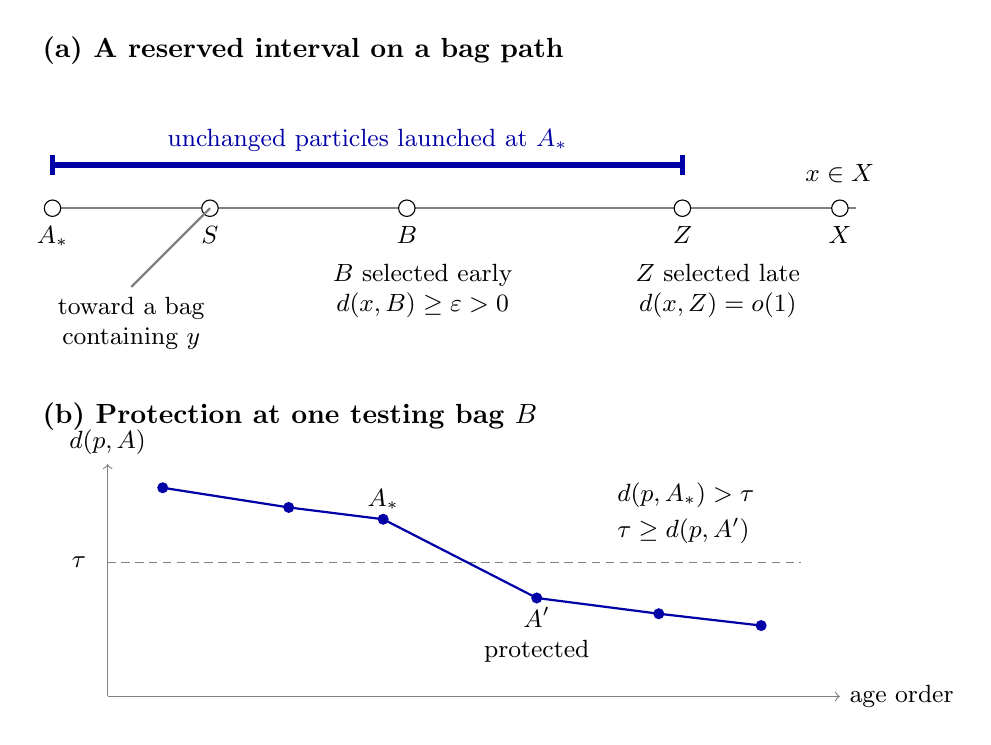
\begin{tikzpicture}[x=1cm,y=1cm,font=\small,
 bag/.style={circle,draw,fill=white,inner sep=2.1pt},
 retained/.style={blue!65!black,line width=2pt}]
 \node[anchor=west,font=\bfseries] at (-.25,2.0) {(a) A reserved interval on a bag path};
 \draw[gray,thick] (0,0)--(10.2,0);
 \foreach \x/\name in {0/A_*,2/S,4.5/B,8/Z,10/X} {
   \node[bag,label=below:$\name$] at (\x,0) {};
 }
 \draw[gray,thick] (2,0)--(1,-1);
 \node[below,align=center] at (1,-1) {toward a bag\\containing $y$};
 \draw[retained] (0,.55)--(8,.55);
 \draw[retained] (0,.42)--(0,.68);
 \draw[retained] (8,.42)--(8,.68);
 \node[blue!65!black,above] at (4,.6) {unchanged particles launched at $A_*$};
 \node[above,align=center] at (4.5,0) {\strut};
 \node[align=center] at (4.7,-1.05) {$B$ selected early\\$d(x,B)\ge\varepsilon>0$};
 \node[align=center] at (8.45,-1.05) {$Z$ selected late\\$d(x,Z)=o(1)$};
 \node[above] at (10,.2) {$x\in X$};
 \node[anchor=west,font=\bfseries] at (-.25,-2.65) {(b) Protection at one testing bag $B$};
 \draw[->,gray] (.7,-6.2)--(10,-6.2) node[right,black] {age order};
 \draw[->,gray] (.7,-6.2)--(.7,-3.25) node[above,black] {$d(p,A)$};
 \draw[gray,densely dashed] (.7,-4.5)--(9.5,-4.5);
 \node[anchor=east] at (.55,-4.5) {$\tau$};
 \draw[blue!65!black,thick] (1.4,-3.55)--(3,-3.8)--(4.2,-3.95)--(6.15,-4.95)--(7.7,-5.15)--(9,-5.3);
 \foreach \x/\y in {1.4/-3.55,3/-3.8,4.2/-3.95,6.15/-4.95,7.7/-5.15,9/-5.3}
  {\fill[blue!65!black] (\x,\y) circle (2pt);}
 \node[above] at (4.2,-3.95) {$A_*$};
 \node[below,align=center] at (6.15,-4.95) {$A'$\\protected};
 \node[anchor=west] at (7.05,-3.65) {$d(p,A_*)>\tau$};
 \node[anchor=west] at (7.05,-4.1) {$\tau\ge d(p,A')$};
\end{tikzpicture}
\caption{The two orders in the anchor argument.
In (a), the selected early bag $B$ and late terminal bag $Z$ lie in the
reservation of $A_*$; the branch toward $y$ makes $B$ a testing bag on
the path to $Z$. The horizontal axis records bag order, not metric
distance, and no first late or last early bag is depicted.
In (b), the entries are ordered by launch time in the list at $B$.
The distance list is nonincreasing. The immediate successor $A'$ is
protected when one of the thresholds $\tau=L/100$ or $\tau=JL$ lies
between its distance and that of $A_*$, where $L=d(p,q)$ is supplied
by Lemma~\ref{lem:anchor-obstruction}. All spacings are schematic.}
\label{fig:anchor-reservations}
\end{figure}


\begin{lemma}[Protection of the immediate successor]
\label{lem:protected-successor}
At any selected early eviction test $B$, suppose the immediate successor
$A'$ of $A_*$ in the inclusive cache list was launched at or after $S$.
Then $A'$ is protected and cannot be evicted at this test.
\end{lemma}

\begin{proof}
Let $p\in B$ be nearest to $x$, and put $\delta=d(x,B)$.
If $A'$ is the current proposal, $d(p,A')=0$.  Otherwise its reservation
lasts from its launch through $B$, and its launch lies on the bag path
from $y$ to $B$.  Equation~\eqref{eq:anchor-launch-test} yields
\[
 b_kd(p,A')\leq D(y,p)\leq D(y,x)+U\delta.
\]
Because $\delta$ is early, $D(y,x)/\delta$ is infinitesimal.  The choice
of $K$ in \eqref{eq:anchor-parameters} consequently gives, eventually,
\begin{equation}\label{eq:successor-distance-bounds}
 d(p,A')\leq K\delta.
\end{equation}
This inequality also holds for a proposal.  Monotonicity of distances
along the path gives $d(x,A')\leq d(x,S)=1$, so in all cases
\begin{equation}\label{eq:successor-absolute-bounds}
 d(p,A')\leq\delta+1\leq2,
 \qquad d(p,A_*)\geq D_0-\delta\geq D_0-1.
\end{equation}

Choose $q$ from Lemma~\ref{lem:anchor-obstruction} and write $L=d(p,q)$.
There are two alternatives.  If $L\leq300$, then
\[
 JL\geq\frac{J\delta}{4}>K\delta\geq d(p,A'),
 \qquad JL\leq300J<H-1<D_0-1\leq d(p,A_*).
\]
If $L>300$, then
\[
 \frac{L}{100}>3>2\geq d(p,A'),
 \qquad \frac{L}{100}\leq\frac{D_0}{10}
       <D_0-1\leq d(p,A_*).
\]
In either case one of the thresholds in \eqref{eq:cache-thresholds}
lies strictly below $d(p,A_*)$ and at or above $d(p,A')$.
Since the distance list is nonincreasing and $A'$ immediately follows
$A_*$, it is precisely the entry protected by this drop.
\end{proof}

\begin{lemma}[A younger crossing anchor exists]
\label{lem:younger-crossing}
Under the normalized failure assumption \eqref{eq:normalized-failure},
there is a crossing anchor younger than $A_*$.
\end{lemma}

\begin{proof}
Inspect the inclusive cache list at the insertion test at $S$.
By Lemma~\ref{lem:old-distant-anchor}, $A_*$ was launched strictly
above $S$, so this is indeed a non-root insertion.  Consider the
younger entries whose launches were strictly above $S$.  Their number
is bounded by $n_0+1$; by a finite ultrafilter alternative, enumerate
them as a fixed finite list of anchor sequences.
These are all the anchors younger than $A_*$ and launched above $S$
that can be present at any later test: an evicted reservation never
returns, and every later launch is at or below $S$.

Each has effective start $S$, which is early.  If any had a late terminal
bag, it would be a crossing anchor younger than $A_*$.  By the choice
of $A_*$, every one must instead have an early terminal bag.  Such a bag
is its actual eviction bag, since the endpoint $X$ is late.

If this finite list is nonempty, take the latest of these eviction
times, say $B_0$.  It is early.  At this test an old younger anchor is
actually evicted, so the new proposal is retained: exactly one entry
is evicted at an insertion.  The anchor $A_*$ remains present, because
its terminal time is late.  Immediately after this eviction no younger
anchor launched above $S$ remains, and the retained proposal ensures
that at least one younger entry exists.  Therefore $A_*$ has an
immediate successor $A'$ whose launch is at or after $S$.

If the finite list is empty, the proposal at $S$ is itself the immediate
successor of $A_*$.  It is retained automatically when there is space;
at a full insertion Lemma~\ref{lem:protected-successor} prohibits its
eviction.  Thus in this case too there is an immediate successor $A'$
launched at or after $S$, present just after an early test $B_0=S$.

Fix this successor $A'$.  Its launch is no later than the early time
$B_0$, so its effective start is early.  If its terminal bag is late,
it is the required younger crossing anchor.  Otherwise its terminal
bag is an early eviction time $B_1$.  The anchor $A_*$ is still present
at $B_1$.  While both anchors remain, $A'$ remains the immediate
successor: there was no entry between them at $B_0$, and all subsequent
insertions are younger than $A'$.  Hence
Lemma~\ref{lem:protected-successor} prohibits eviction of $A'$ at
$B_1$, a contradiction.

This argument selected only a bounded list of anchors, its last
eviction, and one successor's terminal time.  It does not use induction
over an unbounded or limiting order of early times.
\end{proof}

\begin{proof}[Proof of Proposition~\ref{prop:combined-lower}]
If no such constant existed, choosing ratios smaller than $1/i$ would
give \eqref{eq:failed-lower-comparison}.  The normalization above and
Lemmas~\ref{lem:youngest-crossing}--\ref{lem:younger-crossing} would then
produce a crossing anchor younger than the youngest crossing anchor.
This contradiction rules out a sequence of ratios tending to zero.
Their infimum over all nontrivial admissible examples and all distinct
pairs is therefore positive.  Choose $\lambda_k$ no larger than that
infimum.  Equal pairs and the one-vertex graph satisfy
\eqref{eq:combined-lower} automatically.
\end{proof}
